% =============================================================================
%  벨만 방정식과 최적성 — 『밑바닥부터 시작하는 딥러닝 4』 3장 정리
%
%  컴파일:  tectonic -X compile ch03_bellman.tex
%  (XeLaTeX 계열 엔진 + kotex + NanumGothic 필요)
% =============================================================================
\documentclass[11pt,a4paper]{article}

\usepackage{kotex}
\usepackage{amsmath,amssymb}
\usepackage{amsthm}
\usepackage{graphicx}
\usepackage{booktabs}
\usepackage{multirow}
\usepackage{listings}
\usepackage{xcolor}
\usepackage{algorithm}
\usepackage{algpseudocode}
\usepackage[margin=27mm,top=28mm,bottom=28mm]{geometry}
\usepackage[labelsep=period,font=small,labelfont=bf]{caption}
\usepackage{enumitem}
\usepackage[hidelinks]{hyperref}

% ---- 한글 글꼴 -------------------------------------------------------------
\setmainhangulfont{NanumGothic}
\setsanshangulfont{NanumGothic}
\setmonohangulfont[Scale=MatchLowercase]{NanumGothic}

% ---- 한글 캡션 이름 ---------------------------------------------------------
\renewcommand{\figurename}{그림}
\renewcommand{\tablename}{표}
\renewcommand{\refname}{참고문헌}
\renewcommand{\abstractname}{초록}
\renewcommand{\contentsname}{차례}
\floatname{algorithm}{알고리즘}
\renewcommand{\algorithmicrequire}{\textbf{입력:}}
\renewcommand{\algorithmicensure}{\textbf{출력:}}

% ---- 정리 환경 -------------------------------------------------------------

% ---- 코드 리스팅 -----------------------------------------------------------
\definecolor{codekw}{RGB}{0,86,153}
\definecolor{codecm}{RGB}{112,128,144}
\definecolor{codestr}{RGB}{163,21,21}
\definecolor{codebg}{RGB}{249,249,250}
% 주의: listings는 라틴 문자를 단어 단위로 버퍼링했다가 출력하는데, kotex 환경에서
% 한글이 섞이면 버퍼가 한글 뒤에 flush되어 글자 순서가 뒤바뀐다("q에" -> "에q").
% 그래서 한글 주석은 escapeinside 구간에서 일반 조판 모드로 넘겨 처리한다.
\lstdefinestyle{py}{
  language=Python,
  escapeinside={<@}{@>},
  basicstyle=\ttfamily\small,
  keywordstyle=\color{codekw}\bfseries,
  commentstyle=\color{codecm}\itshape,
  stringstyle=\color{codestr},
  backgroundcolor=\color{codebg},
  frame=single,
  rulecolor=\color{black!25},
  framesep=5pt,
  columns=fullflexible,
  keepspaces=true,
  showstringspaces=false,
  breaklines=true,
  captionpos=b,
  numbers=none,
  aboveskip=1.1em,
  belowskip=0.6em,
}
\lstset{style=py}
\renewcommand{\lstlistingname}{코드}

% ---- 그림 경로 -------------------------------------------------------------
\graphicspath{{../../images/figures/}{../../images/equations/}{../images/}}

% ---- 편의 매크로 -----------------------------------------------------------
\newcommand{\E}{\mathbb{E}}
\newcommand{\Sset}{\mathcal{S}}
\newcommand{\Aset}{\mathcal{A}}
\newcommand{\Lone}{\texttt{L1}}
\newcommand{\Ltwo}{\texttt{L2}}
\newcommand{\bookfig}[1]{\textit{출처: 원서 그림 #1.}}
\newcommand{\cmt}[1]{\textcolor{codecm}{#1}}   % 리스팅 안의 한글 주석

% ---- 절 번호를 원서 3장 목차에 맞춤 -----------------------------------------
% 번호 있는 절은 원서/README의 3.1~3.6과 정확히 대응한다. 서론과 재현 정보는
% 번호를 붙이지 않고, 하위 절보다 깊은 제목은 번호와 차례에서 뺀다.
\renewcommand{\thesection}{3.\arabic{section}}
\setcounter{secnumdepth}{2}
\setcounter{tocdepth}{2}

\title{\bfseries 벨만 방정식과 최적성\\[2mm]
\large 무한한 미래를 유한한 연립방정식으로 바꾸는 재귀 구조, 그리고 $\max$가 들어올 때 달라지는 것}
\author{sajacaros\\\small \texttt{sajacall82@naver.com}}
\date{2026년 8월 25일}

\begin{document}
\maketitle

\begin{abstract}
\noindent
앞 장에서 마르코프 결정 과정의 목표를 상태 가치 함수 $v_\pi(s)=\E_\pi[G_t\mid S_t=s]$로 정의하였으나,
이를 정의대로 계산하려면 무한히 이어지는 궤적을 모두 펼쳐야 하고 최적 정책을 찾으려면 $|\Aset|^{|\Sset|}$개의
정책을 모두 평가해야 했다. \emph{벨만 방정식}(Bellman equation)은 이 두 벽을 동시에 허문다. 수익의 재귀
구조 $G_t=R_t+\gamma G_{t+1}$ 한 줄에서 출발하여, 무한한 미래를 ``한 걸음의 보상 $+$ 이웃 상태의 가치''로
접어 넣으면 가치 함수는 미지수 $|\Sset|$개짜리 연립일차방정식의 해가 된다.
본고는 이 도출을 백업 다이어그램의 확률 셈법에서부터 따라간 뒤, 행동 가치 함수 $q_\pi(s,a)$를 경유하여
$\sum_a\pi(a\mid s)$를 $\max_a$로 바꾼 벨만 최적 방정식에 이르는 경로를 정리한다.
원서\cite{dlfs4} 3장은 수식 중심이어서 실행 가능한 코드를 제공하지 않으므로, 두 칸짜리 그리드 월드와
$3\times4$ 그리드 월드를 소재로 예제 네 편을 구성하였다. 본고의 절 구성은 원서 3장의 목차를 그대로
따르며, 원서에 없는 논의는 별도의 절로 떼지 않고 그것이 필요해지는 자리의 본문에 ``[보충]''으로 표시해
두었다. 그렇게 남긴 것은 셋이며, 그 가운데 둘이 다음 장으로 곧장 이어진다. 첫째, 무작위 정책의 $Q$를
한 번 탐욕화하면 $3\times4$ 그리드의 10개 상태 \emph{전부}에서 가치가 오르지만
(평균 $-0.212\to0.760$) 세 상태는 여전히 최적($0.826$)에 못 미쳐,
``한 번의 탐욕화''와 ``반복''을 가르는 간극이 수치로 드러난다. 둘째, 벨만 최적 방정식의 손풀이가
전제한 네 가지 결정적 정책 가정 중 자기일관인 것이 하나뿐임을 전수 확인하여, $\max$를 임의로 지운 식의
해는 최적 가치가 아니라 그 나쁜 정책의 가치일 뿐임을 보인다.

\vspace{2mm}
\noindent\textbf{주제어:} 강화 학습, 벨만 방정식, 벨만 최적 방정식, 행동 가치 함수, 연립일차방정식,
반복 대입, 고정점, 탐욕 정책
\end{abstract}

\tableofcontents
\vspace{4mm}

% =============================================================================
\section*{서론}
\addcontentsline{toc}{section}{서론}
% =============================================================================

\subsection*{전수 탐색의 벽}

앞 장\cite{ch02}에서 마르코프 결정 과정(MDP)을 정식화하고 목표를 상태 가치 함수
\begin{equation}
  v_\pi(s) = \E_\pi\bigl[G_t \mid S_t=s\bigr],
  \qquad
  G_t = R_t + \gamma R_{t+1} + \gamma^2 R_{t+2} + \cdots
  \label{eq:value-def}
\end{equation}
로 정의하였다. 그리고 두 칸짜리 그리드 월드에서 최적 정책을 찾을 때는 결정적 정책 네 가지를 모두
나열하여 각각의 가치를 500걸음 시뮬레이션으로 재는 전수 탐색을 썼다.

이 방법은 두 군데에서 막힌다. 하나는 \emph{정책 하나의 가치를 재는 일}이 끝나지 않는다는 것이다.
식~\eqref{eq:value-def}의 $G_t$는 무한급수이므로 정의대로는 끝까지 더할 수 없고, 500걸음에서 자르는 것은
어디까지나 근사다. 다른 하나는 \emph{재야 할 정책의 수}다. 결정적 정책의 수는 $|\Aset|^{|\Sset|}$이므로
상태가 100개이고 행동이 4가지면 $4^{100}\approx1.6\times10^{60}$가지를 세어야 한다. 두 칸 세계에서 네
가지를 세어 본 것은 문제가 작았기 때문이지 방법이 좋았기 때문이 아니다.

그림~\ref{fig:backup-infinite}이 첫 번째 벽을 그대로 보여준다. 앞 장에서 그린 백업 다이어그램인데,
맨 아래에서 가지가 점선으로 계속 이어진다. 수익을 정의대로 구하려면 이 점선을 끝까지 따라가야 한다.

\begin{figure}[htbp]
\centering
\includegraphics[width=0.86\linewidth]{{fig 3-1}.png}
\caption{결정적 정책(왼쪽)과 확률적 정책(오른쪽)의 백업 다이어그램. 맨 아래에서 가지가 점선으로 계속
이어지는 것이 문제다. 벨만 방정식의 발상은 \emph{한 단계만 내려가고 그 아래 전체를 가치 함수 하나로
대신하는 것}이다. \bookfig{3-1}}
\label{fig:backup-infinite}
\end{figure}

벨만 방정식의 착상은 단순하다. 점선 아래에 있는 것도 결국 ``그 상태에서 시작하는 수익의 기댓값''이므로
$v_\pi(s')$ 자체다. 그렇다면 무한한 가지를 펼치는 대신 한 층만 내려간 뒤 나머지를 $v_\pi(s')$로 바꿔 쓰면
된다. 그 대가로 $v_\pi$가 등식의 양변에 나타나지만, 그것은 무한급수가 아니라 유한한 연립방정식이다.

\subsection*{본고의 구성과 기여}

본고는 원서 3장의 목차를 그대로 따른다. \S\ref{sec:derivation}에서 백업 다이어그램의 확률 셈법을
정리한 뒤 수익의 재귀 구조로부터 벨만 방정식을 도출하고, \S\ref{sec:linear}에서 그 식을 두 칸 세계와
$3\times4$ 그리드에 적용하여 연립일차방정식으로 푼다. \S\ref{sec:qsec}에서 행동 가치 함수를 도입하여
$V$와 $Q$의 상호 변환을 정리하고, \S\ref{sec:opt}에서 $\sum_a\pi(a\mid s)$를 $\max_a$로 바꾼 벨만 최적
방정식을 세운 뒤 \S\ref{sec:opt-example}에서 그것을 다시 두 칸 세계에 적용한다.
\S\ref{sec:summary}이 정리다.

원서 3장에는 소스 코드가 없으므로 예제 네 편을 새로 구성하였다(표~\ref{tab:code}). 원서에 없는 논의는
절을 따로 만들어 밀어 두지 않고, 그것이 필요해지는 자리의 본문에 ``[보충]''으로 표시해 두었다. 그렇게
남긴 것은 셋이다. \S\ref{sec:significance} 끝에서는 정확해를 주는 직접 해법을 두고도 다음 장이 왜
반복법으로 가는지를 연산량과 기억 용량으로 견준다. \S\ref{sec:q-bellman-sec} 끝에서는 $3\times4$
그리드의 $Q$를 한 번 탐욕화해 보는데, 4장 정책 반복법이 왜 ``한 번''이 아니라 ``반복''인지가 거기서
나온다. \S\ref{sec:opt-apply} 끝에서는 손풀이가 전제한 네 가지 가정을 전부 풀어, 벨만 최적 방정식을
푼다는 일의 논리 구조를 드러낸다.

반면 축소 사상의 형식적 증명, 수렴률의 고윳값 분해, 손익분기 상태 수의 닫힌 식 같은 논의는 이 장의
줄거리를 따라가는 데 꼭 필요하지 않아 덜어냈다. 반복 대입이 왜 통하는지는 \S\ref{sec:significance}에서
``오차가 한 걸음마다 $\gamma$배 이하로 줄어든다''는 사실과 고정점이라는 말로만 짚고 넘어간다.

% =============================================================================
\section{벨만 방정식 도출}
\label{sec:derivation}
% =============================================================================

\subsection{확률과 기댓값(사전 준비)}
\label{sec:expectation}

벨만 방정식은 결국 기댓값 계산이므로, 먼저 백업 다이어그램에서 기댓값을 읽는 연습을 해 둔다.
가장 단순한 예는 주사위 한 번 던지기다.

\begin{figure}[htbp]
\centering
\includegraphics[width=0.56\linewidth]{{fig 3-2}.png}
\caption{주사위 한 번 던지기의 백업 다이어그램. 검은 점에서 여섯 갈래로 뻗고 가지마다 확률 $1/6$이
붙는다. \bookfig{3-2}}
\label{fig:dice}
\end{figure}

가지에 붙은 확률과 끝의 값을 곱해 모두 더한 것이 기댓값이다.
\begin{equation}
  \E[X] = \sum_x x\,p(x) = \frac{1+2+3+4+5+6}{6} = 3.5.
\end{equation}

다음은 두 단계짜리 문제다. 주사위를 던져 홀수가 나오면 공정한 동전을, 짝수가 나오면 앞면이 잘 나오는
동전을 던진다. 동전이 앞면이면 주사위 눈만큼 보상을 받고 뒷면이면 $0$이다.

\begin{figure}[htbp]
\centering
\begin{minipage}[t]{0.46\linewidth}\centering
  \includegraphics[width=\linewidth]{{fig 3-3}.png}
\end{minipage}\hfill
\begin{minipage}[t]{0.50\linewidth}\centering
  \includegraphics[width=\linewidth]{{fig 3-4}.png}
\end{minipage}
\caption{두 단계짜리 문제(왼쪽)와 이를 하나의 백업 다이어그램으로 편 것(오른쪽). 두 번째 단계의 확률이
첫 번째 단계의 결과에 \emph{의존}한다는 점이 MDP와 같은 구조다. 홀수 가지의 앞면 확률은 $1/2$,
짝수 가지는 $4/5$이다. \bookfig{3-3, 3-4}}
\label{fig:two-stage}
\end{figure}

이때 기댓값은 맨 위에서 맨 아래까지 가지의 확률을 모두 곱하고 거기에 마지막 값을 곱해 더한 것이다.
\begin{align}
  \E[R] &= \tfrac16\Bigl(1\cdot\tfrac12 + 2\cdot\tfrac45 + 3\cdot\tfrac12
           + 4\cdot\tfrac45 + 5\cdot\tfrac12 + 6\cdot\tfrac45\Bigr) \notag\\
        &= \tfrac16\bigl(0.5+1.6+1.5+3.2+2.5+4.8\bigr) = \frac{14.1}{6} = 2.35.
  \label{eq:two-stage}
\end{align}
뒷면 가지는 보상이 $0$이라 합에서 사라지므로 12개 가지 중 6개 항만 남았다.

식~\eqref{eq:two-stage}에서 확인할 것은 두 가지다. 첫째, \emph{가지를 따라 확률을 곱해 더한다}는 셈법이
층이 늘어도 그대로 통한다. 둘째, 두 번째 층의 확률이 첫 번째 층의 결과에 따라 달라진다. 이 두 성질이
그대로 벨만 방정식의 유도에 쓰인다. MDP에서는 첫 번째 층이 정책이고 두 번째 층이 상태 전이일 뿐이다.

\subsection{벨만 방정식 도출}
\label{sec:bellman-derive}

\subsubsection{수익의 재귀 구조}

출발점은 수익의 정의다.
\begin{equation}
  G_t = R_t + \gamma R_{t+1} + \gamma^2 R_{t+2} + \gamma^3 R_{t+3} + \cdots
  \label{eq:return}
\end{equation}
한 시각 뒤의 수익도 같은 모양이다.
\begin{equation}
  G_{t+1} = R_{t+1} + \gamma R_{t+2} + \gamma^2 R_{t+3} + \cdots
  \label{eq:return-next}
\end{equation}
식~\eqref{eq:return}에서 첫 항을 떼고 나머지를 $\gamma$로 묶으면 식~\eqref{eq:return-next}이 그대로
나타난다.
\begin{equation}
  \boxed{\;G_t = R_t + \gamma G_{t+1}.\;}
  \label{eq:return-recursive}
\end{equation}

이 한 줄에서 이 장의 모든 식이 나온다. 식~\eqref{eq:return-recursive}이 하는 일은 무한히 이어지는 합을
\emph{한 걸음}과 \emph{나머지 전부}로 나눈 것뿐이지만, 나머지 전부가 원래 문제와 같은 모양이라는 점이
결정적이다. 앞 장에서 이 식은 보상 열을 뒤에서부터 접어 올리는 계산 요령으로만 쓰였는데, 이제 그것이
방정식이 된다.

이제 식~\eqref{eq:return-recursive}을 가치 함수의 정의
\begin{equation}
  v_\pi(s) = \E_\pi\bigl[G_t \mid S_t=s\bigr]
  \label{eq:v-def}
\end{equation}
에 대입하고 기댓값의 선형성으로 두 항을 나눈다.
\begin{equation}
  v_\pi(s) = \E_\pi\bigl[R_t \mid S_t=s\bigr] + \gamma\,\E_\pi\bigl[G_{t+1} \mid S_t=s\bigr].
  \label{eq:v-split}
\end{equation}

\begin{figure}[htbp]
\centering
\includegraphics[width=0.72\linewidth]{{fig 3-6}.png}
\caption{식~\eqref{eq:v-split}의 두 항. 하늘색으로 칠해진 두 덩어리를 각각 전개한다. 왼쪽은 한 걸음의
기댓값이므로 \S\ref{sec:expectation}의 셈법을 그대로 적용하면 되고, 오른쪽은 그 뒤에 처리한다.
\bookfig{3-6}}
\label{fig:two-terms}
\end{figure}

\subsubsection{두 층의 확률: 정책과 상태 전이}

식~\eqref{eq:v-split}의 두 항을 전개하려면 어떤 확률이 걸려 있는지 알아야 한다. 그림~\ref{fig:two-layers}이
그것을 보여준다.

\begin{figure}[htbp]
\centering
\includegraphics[width=0.66\linewidth]{{fig 3-5}.png}
\caption{한 걸음에 걸린 두 개의 확률분포. 하늘색(상태 $\to$ 행동)은 \emph{정책} $\pi(a\mid s)$이고,
주황색(행동 $\to$ 다음 상태)은 \emph{상태 전이 확률} $p(s'\mid s,a)$다. 왼쪽의 막대그래프 두 개는
각각이 확률분포임을 강조한 것이다. \bookfig{3-5}}
\label{fig:two-layers}
\end{figure}

\S\ref{sec:expectation}의 두 단계 문제와 구조가 같다. 맨 위에서 $s'$까지 내려가는 한 가지의 확률은
두 층의 확률을 곱한 $\pi(a\mid s)\,p(s'\mid s,a)$이고, 그 끝에 붙은 값이 보상 $r(s,a,s')$이다.
따라서 식~\eqref{eq:v-split}의 첫 항은
\begin{equation}
  \E_\pi\bigl[R_t \mid S_t=s\bigr]
  = \sum_{a}\sum_{s'} \pi(a\mid s)\,p(s'\mid s,a)\,r(s,a,s')
  \label{eq:first-term}
\end{equation}
이 된다. 둘째 항도 같다. 상태가 $s'$으로 바뀌고 나면 그 뒤의 기대 수익은 정의상 $v_\pi(s')$이므로
\begin{equation}
  \E_\pi\bigl[G_{t+1} \mid S_t=s\bigr]
  = \sum_{a}\sum_{s'} \pi(a\mid s)\,p(s'\mid s,a)\,v_\pi(s')
  \label{eq:second-term}
\end{equation}
이다. 여기가 유도의 핵심이다. $G_{t+1}$은 그 자체로 무한급수인데, 그 무한급수의 기댓값을 다시 펼치지
않고 $v_\pi(s')$이라는 \emph{이름}으로 대신했다. 그림~\ref{fig:backup-infinite}의 점선이 여기서 잘린다.

\subsubsection{벨만 방정식}

식~\eqref{eq:first-term}과 \eqref{eq:second-term}을 식~\eqref{eq:v-split}에 넣고 공통의 $\sum$으로 묶으면
\emph{벨만 방정식}을 얻는다.
\begin{equation}
  \boxed{\;
  v_\pi(s) = \sum_{a}\sum_{s'} \pi(a\mid s)\,p(s'\mid s,a)
             \bigl\{\, r(s,a,s') + \gamma\, v_\pi(s') \,\bigr\}.
  \;}
  \label{eq:bellman}
\end{equation}
이중 합을 안팎으로 분리해 쓰면 코드로 옮기기 좋은 형태가 된다.
\begin{equation}
  v_\pi(s) = \sum_{a} \pi(a\mid s) \sum_{s'} p(s'\mid s,a)
             \bigl\{\, r(s,a,s') + \gamma\, v_\pi(s') \,\bigr\}.
  \label{eq:bellman-nested}
\end{equation}
바깥쪽 $\sum_a$는 정책에 대한 평균이고 안쪽 $\sum_{s'}$은 상태 전이에 대한 평균이다.

상태 전이가 결정적이어서 $s'=f(s,a)$로 정해지면 안쪽 합이 사라진다.
\begin{equation}
  v_\pi(s) = \sum_{a} \pi(a\mid s)
             \bigl\{\, r\bigl(s,a,f(s,a)\bigr) + \gamma\, v_\pi\bigl(f(s,a)\bigr) \,\bigr\}.
  \label{eq:bellman-det}
\end{equation}
본고가 다루는 두 환경은 모두 상태 전이가 결정적이므로 실제 계산에는 식~\eqref{eq:bellman-det}을 쓴다.

식~\eqref{eq:bellman}이 말하는 바는 한 문장으로 줄어든다.
\begin{center}
\emph{어떤 상태의 가치는 (한 걸음 보상의 기댓값) $+$ $\gamma\,\times$ (이웃 상태 가치의 기댓값)이다.}
\end{center}
무한한 미래를 다 볼 필요가 없어졌다는 것이 얻은 것이고, $v_\pi$가 좌변과 우변에 동시에 나타나는
자기참조 구조가 치른 대가다. 다음 절에서 보듯 그 대가는 연립방정식을 푸는 정도의 값이다.

% =============================================================================
\section{벨만 방정식의 예}
\label{sec:linear}
% =============================================================================

\subsection{두 칸짜리 그리드 월드}
\label{sec:two-square}

앞 장에서 쓴 두 칸짜리 그리드 월드를 그대로 가져온다. 이번에 평가할 정책은
$\Lone$과 $\Ltwo$ 어디에서나 \texttt{Left}와 \texttt{Right}를 $0.5$씩 고르는 무작위 정책이다.

\begin{figure}[htbp]
\centering
\begin{minipage}[t]{0.44\linewidth}\centering
  \includegraphics[width=\linewidth]{{fig 3-7}.png}
\end{minipage}\hfill
\begin{minipage}[t]{0.52\linewidth}\centering
  \includegraphics[width=\linewidth]{{fig 3-8}.png}
\end{minipage}
\caption{두 칸짜리 그리드 월드와 무작위 정책(왼쪽), 그 백업 다이어그램(오른쪽). 왼쪽 막대그래프 두 개의
높이가 같은 것이 $\pi(a\mid s)=0.5$이다. 오른쪽에서 상태에서 나오는 가지는 둘로 갈라지지만 \emph{행동에서
나오는 화살표는 하나뿐}인데, 이것이 상태 전이가 결정적이라는 뜻이며 따라서 식~\eqref{eq:bellman-det}을
쓸 수 있다. \bookfig{3-7, 3-8}}
\label{fig:two-square}
\end{figure}

환경의 규칙은 앞 장과 같다. 벽에 부딪히면 $-1$, $\Ltwo$로 이동하면 사과를 먹어 $+1$, $\Ltwo$에서 $\Lone$로
가면 $0$이며 $\gamma=0.9$다. 이제 상태마다 벨만 방정식을 한 줄씩 세운다.

\begin{figure}[htbp]
\centering
\begin{minipage}[t]{0.48\linewidth}\centering
  \includegraphics[width=\linewidth]{{fig 3-9}.png}
\end{minipage}\hfill
\begin{minipage}[t]{0.48\linewidth}\centering
  \includegraphics[width=\linewidth]{{fig 3-10}.png}
\end{minipage}
\caption{$v_\pi(\Lone)$(왼쪽)과 $v_\pi(\Ltwo)$(오른쪽)에 대한 한 단계짜리 다이어그램. 그림~\ref{fig:two-square}
오른쪽의 맨 윗부분만 떼어낸 것으로, 아래가 점선으로 이어지지 않고 $\Lone$, $\Ltwo$에서 \emph{끊겨} 있다.
그 아래 전체를 $v_\pi(\Lone)$, $v_\pi(\Ltwo)$로 대신하는 것이 벨만 방정식의 요령이다. \bookfig{3-9, 3-10}}
\label{fig:one-step}
\end{figure}

그림~\ref{fig:one-step}을 그대로 읽으면 다음 두 식이 나온다.
\begin{align}
  v_\pi(\Lone) &= 0.5\bigl\{-1 + 0.9\,v_\pi(\Lone)\bigr\} + 0.5\bigl\{\,1 + 0.9\,v_\pi(\Ltwo)\bigr\}, \\
  v_\pi(\Ltwo) &= 0.5\bigl\{\;\;0 + 0.9\,v_\pi(\Lone)\bigr\} + 0.5\bigl\{-1 + 0.9\,v_\pi(\Ltwo)\bigr\}.
\end{align}
정리하면 미지수 두 개짜리 연립일차방정식이다.
\begin{equation}
  \left\{
  \begin{aligned}
    -0.55\,v_\pi(\Lone) + 0.45\,v_\pi(\Ltwo) &= 0,\\
     0.45\,v_\pi(\Lone) - 0.55\,v_\pi(\Ltwo) &= 0.5.
  \end{aligned}
  \right.
  \label{eq:two-eqs}
\end{equation}
풀면 $v_\pi(\Lone)=-2.25$, $v_\pi(\Ltwo)=-2.75$다. 무작위로 걸으면 벽에 부딪히는 일이 잦아 값이 음수가
된다.

식~\eqref{eq:two-eqs}을 세운 과정은 정책이 바뀌어도 달라지지 않는다. 앞 장이 전수 탐색으로 찾아낸
결정적 정책 $\mu=(\texttt{Right},\texttt{Left})$에 대해 같은 자리에 다른 확률과 보상을 넣어 두 식을
세우고 풀면 표~\ref{tab:two-square-values}의 아래 행이 나온다. 예제
\texttt{s01\_bellman\_linear.py}가 두 정책의 연립방정식을 모두 풀어 확인한다.

\begin{table}[htbp]
\centering
\caption{두 칸짜리 그리드 월드의 상태 가치($\gamma=0.9$). 무작위 정책의 값은 식~\eqref{eq:two-eqs}의 해와
같고, 결정적 정책 $\mu$의 값은 앞 장이 500걸음 시뮬레이션으로 얻었던 값과 같다.}
\label{tab:two-square-values}
\small
\begin{tabular}{@{}lccl@{}}
\toprule
정책 & $v(\Lone)$ & $v(\Ltwo)$ & 비고 \\
\midrule
무작위 $\pi(a\mid s)=0.5$                       & $-2.2500$ & $-2.7500$ & 원서 3.2절의 값 \\
$\mu=(\texttt{Right},\texttt{Left})$            & $5.2632$  & $4.7368$  & 앞 장의 전수 탐색 최적 정책 \\
\bottomrule
\end{tabular}
\end{table}

표~\ref{tab:two-square-values}의 아래 행이 이 장의 요점이다. 앞 장에서 $5.2632$를 얻으려면 정책을 고정하고
500걸음을 시뮬레이션해야 했다. 여기서는 $2\times2$ 연립방정식을 한 번 풀었다. 근사가 정확해로 바뀌었고
걸음 수라는 임의의 절단 지점도 사라졌다.

\subsubsection{\texorpdfstring{$3\times4$}{3x4} 그리드 월드로}

상태가 12개가 되면 손으로 풀 수 있는 크기를 넘어서지만, 세우는 방법은 조금도 달라지지 않는다. 상태마다
식을 한 줄씩 쓰면 미지수 12개짜리 연립일차방정식이고, 같은 예제의 후반부가 그것을 푼다. 이 환경은 다음
장에서 반복 계산으로 다시 풀 문제다.

\begin{table}[htbp]
\centering
\caption{$3\times4$ 그리드 월드에서 무작위 정책($\pi(a\mid s)=0.25$)의 상태 가치($\gamma=0.9$).
$(0,3)$은 목표 상태(가치 $0$), $(1,1)$은 벽, $(1,3)$은 폭탄이다. 12원 연립방정식의 정확해다.}
\label{tab:grid-random}
\small
\begin{tabular}{@{}lrrrr@{}}
\toprule
 & $w=0$ & $w=1$ & $w=2$ & $w=3$ \\
\midrule
$h=0$ & $0.0257$  & $0.0946$  & $0.2055$  & $0.0000$ \\
$h=1$ & $-0.0318$ & \textit{(벽)} & $-0.4980$ & $-0.3727$ \\
$h=2$ & $-0.1034$ & $-0.2210$ & $-0.4368$ & $-0.7857$ \\
\bottomrule
\end{tabular}
\end{table}

표~\ref{tab:grid-random}에서 오른쪽 아래 $-0.7857$이 가장 낮다. 폭탄$(1,3)$ 바로 아래이면서 목표에서
멀어, 무작위로 걸으면 폭탄에 빨려 들어갈 확률이 높은 자리다. 목표 상태 왼쪽의 $0.2055$가 가장 높은 것도
같은 이유의 뒤집힌 표현이다.

이 값들은 다음 장의 반복 정책 평가가 구하는 값과 최대 오차 $4.644\times10^{-10}$로 일치한다. 반복 계산에
쓴 종료 문턱이 $10^{-10}$이었으므로 이는 두 방법이 같은 방정식을 서로 다른 방식으로 푼 것임을 보여준다.

\subsection{벨만 방정식의 의의}
\label{sec:significance}

벨만 방정식이 없다면 가치를 구하는 길은 두 가지뿐이고 둘 다 막혀 있다.

\begin{table}[htbp]
\centering
\caption{벨만 방정식이 없을 때 $v_\pi(s)$에 이르는 두 경로. 어느 쪽도 끝나지 않는다.}
\label{tab:no-bellman}
\small
\begin{tabular}{@{}ll@{}}
\toprule
방법 & 막히는 곳 \\
\midrule
수익의 정의대로 계산    & 무한히 이어지는 항을 모두 더해야 한다(앞 장은 500걸음에서 잘랐다) \\
모든 궤적을 나열해 기댓값 & 그림~\ref{fig:two-square} 오른쪽처럼 가지가 $2^n$으로 폭발한다 \\
\bottomrule
\end{tabular}
\end{table}

벨만 방정식은 이 문제를 미지수 $|\Sset|$개짜리 \emph{연립일차방정식}으로 바꾼다. 상태가 100개면 100원
연립방정식이며, 유한하고 컴퓨터가 곧바로 풀 수 있는 크기다. 앞 장의 전수 탐색이 마주한 $4^{100}$과는
차원이 다르다. 무한급수와 지수적 나열이라는 두 벽이 동시에 사라지는 자리가 여기다.

다만 정확해를 주는 이 길에도 한계가 있다. 미지수가 $|\Sset|$개인 연립방정식을 정면으로 소거해 푸는 데는
계수를 담을 $|\Sset|\times|\Sset|$ 크기의 표가 필요하고 연산량이 $O(|\Sset|^3)$이므로, 상태가 아주
많아지면 감당하기 어려워진다. 그래서 실제로는 우변에 계속 대입해 근사해로 다가가는 \emph{반복 대입}을 쓰며, 그것이 다음 장의
동적 프로그래밍이다.

반복 대입이 왜 되는지는 벨만 방정식(식~\eqref{eq:bellman})을 다시 보면 알 수 있다. 이 식은 좌변에도
$v_\pi$가 있고 우변에도 $v_\pi$가 있다. $x=f(x)$처럼 \emph{넣은 것이 그대로 다시 나오는} 꼴의 방정식을
\emph{고정점 방정식}이라 하고, 그것을 만족하는 $x$를 $f$의 \emph{고정점}(fixed point)이라 한다. 익숙한
예가 $x=\cos x$다. 계산기에 아무 수나 넣고 $\cos$을 계속 누르면 $0.739085\ldots$로 빨려 들어가는데, 그
값이 $\cos$의 고정점이다.

벨만 방정식을 푸는 일도 이와 같다. 다루는 것이 숫자 하나가 아니라 상태마다 값이 하나씩 적힌 \emph{표},
곧 길이 $|\Sset|$짜리 벡터라는 점만 다르다. 지금 손에 든 표 $v_k$를 \emph{잠정적인} 가치 추정치로 믿고
식~\eqref{eq:bellman}의 우변에 넣어 보자. 상태 $s$에서 한 걸음만 실제로 굴려 보상 $r(s,a,s')$을 받은
다음, 그 이후는 도착한 칸의 값 $v_k(s')$을 그대로 갖다 쓰는 계산이다. 요컨대 \emph{한 걸음은 진짜로
계산하고 나머지는 지금의 추정치로 때우는} 것이며, 그 결과를 모든 상태에 대해 적어 놓은 새 표가
$v_{k+1}$이다.
\begin{equation}
  v_{k+1}(s) = \sum_a \pi(a\mid s)\sum_{s'} p(s'\mid s,a)\bigl\{r(s,a,s')+\gamma\, v_k(s')\bigr\}
  \label{eq:iteration}
\end{equation}
참값 $v_\pi$를 넣었다면 때운 부분까지 참값이므로 나온 표도 $v_\pi$다. 즉 $v_\pi$는 이 되풀이의
고정점이고, $\cos$의 예가 그랬듯이 아무 표에서 출발해 계속 대입하는 것만으로 그 표에 이를 수 있다.

다만 아무 $f$에서나 되는 것은 아니고 $f$가 \emph{두 점 사이의 거리를 줄이는} 함수여야 하는데($\cos$이
그렇다), 식~\eqref{eq:iteration}의 우변이 바로 그런 함수다. 서로 다른 표를 두 개 넣어 보면 알 수 있다.
$v_k$가 들어가는 자리는 $\gamma\,v_k(s')$ 하나뿐이고, 그 앞에 붙은 $\sum_a\pi(a\mid s)\sum_{s'}p(s'\mid s,a)$는
합이 $1$인 확률로 평균을 내는 일이다. 두 표의 차이를 아무리 섞어 평균내도 그중 가장 큰 차이보다 커질 수
없으므로, 남는 것은 앞에 붙은 $\gamma$다. 즉 한 번 대입할 때마다
두 표의 거리는 $\gamma$배 이하로 줄어들며, 그 두 표 중 하나를 참값 $v_\pi$로 두면 오차에 대한 다음 식이
된다.
\begin{equation}
  \|v_k - v_\pi\|_\infty \;\le\; \gamma^{k}\,\|v_0 - v_\pi\|_\infty
  \label{eq:error-bound}
\end{equation}

이 반복을 실제로 돌려 보는 예제가 \texttt{s02\_bellman\_iterative.py}이고 그림~\ref{fig:iterative}이 그
오차다. 로그 눈금에서 직선이라는 것은 오차가 지수적으로 줄어든다는 뜻이고, 그 기울기를 정하는 것이
$\gamma$다. $\gamma$가 $1$에 가까울수록 선이 완만해져 반복이 오래 걸린다는 사실이 두 그림의 차이에 그대로
나타난다.

\begin{figure}[htbp]
\centering
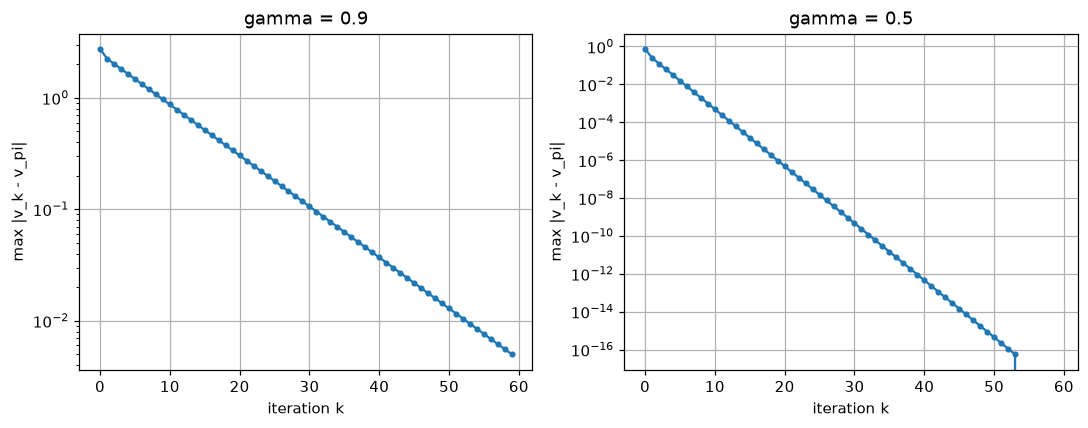
\includegraphics[width=\linewidth]{s02_bellman_iterative.png}
\caption{반복 대입의 오차(로그 눈금). 왼쪽($\gamma=0.9$)은 60회를 돌려도 오차가 $4.5\times10^{-3}$ 남지만,
오른쪽($\gamma=0.5$)은 53회 부근에서 선이 끊긴다. 그 지점이 $0.5^{k}$가 배정밀도로 표현할 수 있는 크기
아래로 내려가 오차가 정확히 $0$이 된 곳이다. \texttt{s02\_bellman\_iterative.py}에서 생성.}
\label{fig:iterative}
\end{figure}

\subsubsection{[보충] 그렇다면 언제 반복법으로 갈아타는가}

직접 해법과 반복법은 주는 것이 서로 다르다. 직접 해법은 정확해를 유한 단계에 주는 대신 $|\Sset|$원
연립방정식을 소거하는 데 $|\Sset|$의 세제곱에 비례하는 연산이 들고, 계수를 담은 $|\Sset|\times|\Sset|$
크기의 표를 통째로 들고 있어야 한다. 반복법은 근사해만 주는 대신 한 번의 갱신 비용이 상태 수에 선형이고, 기억할
것은 길이 $|\Sset|$의 벡터 두 개뿐이며, 필요한 정확도만큼만 돌면 된다.

예제 \texttt{s01\_bellman\_linear.py}가 직접 해법을 쓴 것은 그래서 옳다. 상태가 2개와 12개뿐인 본고의
두 환경은 그 우위가 분명한 크기다. 그러나 이 우위는 세제곱으로 커지는 항에 기대고 있어 금세 뒤집힌다. 먼저 무너지는 쪽은 시간이 아니라 공간이다. $|\Sset|=10^4$이면 계수 표 하나가 배정밀도로
$0.8$\,GB이고 $|\Sset|=10^6$이면 $8$\,TB라 어떤 기계에도 올라가지 않는 반면, 반복법이 들고 있어야 하는
것은 여전히 벡터 두 개다. 다음 장의 동적 프로그래밍이 반복법을 택하는 이유가 여기에 있고, 5장 이후
상태 공간이 더 커질 때 가치 함수를 신경망으로 근사하게 되는 출발점도 같은 자리다.

% =============================================================================
\section{행동 가치 함수(Q 함수)와 벨만 방정식}
\label{sec:qsec}
% =============================================================================

\subsection{행동 가치 함수}
\label{sec:q-def-sec}

지금까지의 $v_\pi(s)$는 ``상태 $s$에서 정책 $\pi$를 따를 때''의 기대 수익이다. 여기서 첫 행동만 정책의
손에서 빼앗아 자유롭게 지정한 것이 \emph{행동 가치 함수}(action-value function), 흔히 $Q$ 함수다.
\begin{equation}
  q_\pi(s,a) = \E_\pi\bigl[G_t \mid S_t=s,\, A_t=a\bigr].
  \label{eq:q-def}
\end{equation}
식~\eqref{eq:v-def}과 비교하면 조건에 $A_t=a$가 하나 더 붙었을 뿐이다.

\begin{figure}[htbp]
\centering
\includegraphics[width=0.78\linewidth]{{fig 3-11}.png}
\caption{$v_\pi$(왼쪽)와 $q_\pi$(오른쪽)의 차이. 주황색으로 감싼 범위가 왼쪽은 상태 $s$만이고 오른쪽은
$s$와 행동 $a$까지다. 왼쪽에서는 첫 행동도 정책이 고르므로 갈래가 여럿이지만, 오른쪽에서는 첫 행동이
지정되어 갈래가 하나로 고정되고 그 아래부터 $\pi$를 따른다. 이 ``첫 행동만 자유''라는 차이가 4장 정책
개선과 6장 Q 러닝의 근거가 된다. \bookfig{3-11}}
\label{fig:v-vs-q}
\end{figure}

$v_\pi$를 유도할 때와 똑같은 순서를 밟는다. 식~\eqref{eq:return-recursive}을 대입하고 선형성으로 나눈 뒤
두 번째 항에 $v_\pi(s')$를 쓰면
\begin{equation}
  \boxed{\;
  q_\pi(s,a) = \sum_{s'} p(s'\mid s,a)\bigl\{\, r(s,a,s') + \gamma\, v_\pi(s') \,\bigr\}
  \;}
  \label{eq:q-from-v}
\end{equation}
를 얻는다. 식~\eqref{eq:bellman-nested}에서 바깥쪽 $\sum_a \pi(a\mid s)$만 떼어낸 모양이다. 정책이
고르던 자리를 우리가 대신 골랐으니 그 평균이 사라지는 것은 당연하다. 반대 방향은 그 평균을 도로
씌우면 된다.
\begin{equation}
  \boxed{\;
  v_\pi(s) = \sum_{a} \pi(a\mid s)\, q_\pi(s,a).
  \;}
  \label{eq:v-from-q}
\end{equation}

식~\eqref{eq:q-from-v}과 \eqref{eq:v-from-q}은 $V$와 $Q$가 같은 정보의 두 표현임을 말한다. 그렇다면 왜
둘 다 필요한가. 표~\ref{tab:v-vs-q}가 그 답이다.

\begin{table}[htbp]
\centering
\caption{$V$와 $Q$의 비교. 마지막 열이 5장 이후 모델 없는 기법이 모두 $Q$를 쓰는 이유다.}
\label{tab:v-vs-q}
\small
\begin{tabular}{@{}llll@{}}
\toprule
 & 입력 & 첫 행동을 고르는 주체 & 행동을 고르려면 \\
\midrule
$v_\pi(s)$    & 상태             & 정책 $\pi$   & $p$와 $r$를 알아야 함(식~\eqref{eq:greedy-v}) \\
$q_\pi(s,a)$  & 상태 $+$ 행동    & \textbf{내가 지정} & $\arg\max_a q_\pi(s,a)$면 끝 \\
\midrule
기억 용량     & $|\Sset|$개      & --- & $|\Sset|\times|\Aset|$개 \\
\bottomrule
\end{tabular}
\end{table}

$Q$는 $|\Aset|$배의 기억 용량을 쓰는 대신, 행동을 고를 때 환경 모델 $p$와 $r$를 참조하지 않아도 되게
해 준다. 환경 모델을 모르는 채로 경험만 가지고 배우는 5장 이후의 기법들이 예외 없이 $Q$를 추정하는
것은 이 한 줄 때문이다.

\subsection{행동 가치 함수를 이용한 벨만 방정식}
\label{sec:q-bellman-sec}

식~\eqref{eq:q-from-v}의 우변에는 아직 $v_\pi$가 남아 있다. 여기에 식~\eqref{eq:v-from-q}을 대입하면
$Q$만으로 닫힌 식이 된다.
\begin{equation}
  \boxed{\;
  q_\pi(s,a) = \sum_{s'} p(s'\mid s,a)\Bigl\{\, r(s,a,s')
               + \gamma \sum_{a'} \pi(a'\mid s')\, q_\pi(s',a') \Bigr\}.
  \;}
  \label{eq:q-bellman}
\end{equation}
식~\eqref{eq:bellman}과 견주면 안쪽에 $\sum_{a'}\pi(a'\mid s')$가 새로 생겼다. \emph{다음 상태에서 고를
행동}까지 정책으로 평균낸다는 뜻이다. 이 부분은 6장 SARSA의 갱신식에 그대로 나타난다.

예제 \texttt{s03\_q\_function.py}가 두 칸 세계에서 이 관계들을 수치로 확인한다.
표~\ref{tab:q-values}가 그 결과다.

\begin{table}[htbp]
\centering
\caption{두 칸짜리 그리드 월드에서 무작위 정책의 $Q$ 함수($\gamma=0.9$). 마지막 열은
식~\eqref{eq:v-from-q}으로 복원한 $v_\pi$이며 표~\ref{tab:two-square-values}의 값과 일치한다.}
\label{tab:q-values}
\small
\begin{tabular}{@{}lrrr@{}}
\toprule
$s$ & $q_\pi(s,\texttt{Left})$ & $q_\pi(s,\texttt{Right})$ & $\tfrac12\bigl(q_\pi(s,\texttt{L})+q_\pi(s,\texttt{R})\bigr) = v_\pi(s)$ \\
\midrule
$\Lone$ & $-3.0250$ & $-1.4750$ & $-2.2500$ \\
$\Ltwo$ & $-2.0250$ & $-3.4750$ & $-2.7500$ \\
\bottomrule
\end{tabular}
\end{table}

표~\ref{tab:q-values}에서 눈여겨볼 것은 $q_\pi(\Lone,\texttt{Right})=-1.4750$이 $v_\pi(\Lone)=-2.2500$보다
\emph{크다}는 점이다. $\Lone$에서 무작위로 고르는 것보다 \texttt{Right}를 고르는 편이 낫다는 뜻이며,
그 차이 $0.775$가 곧 개선의 여지다. $\Ltwo$에서도 \texttt{Left}$(-2.0250)$가 평균$(-2.7500)$보다 낫다.
$V$만 들여다볼 때는 보이지 않던 ``어느 방향으로 고치면 되는가''가 $Q$에서는 표를 훑는 것만으로 읽힌다.

\subsubsection{[보충] 한 번의 탐욕화가 주는 것과 주지 못하는 것}

그렇다면 $Q$를 한 번 탐욕화하면 얼마나 좋아지는가. $3\times4$ 그리드에서 무작위 정책의
$q_\pi$(표~\ref{tab:grid-random}의 $v_\pi$로부터 식~\eqref{eq:q-from-v}로 얻은 것)를 탐욕화한 정책
$\pi'(s)=\arg\max_a q_\pi(s,a)$을 만들고, 그 정책의 가치 $v_{\pi'}$를 다시 연립방정식으로 정확히 풀어
비교하였다. 표~\ref{tab:greedy}가 결과다.

\begin{table}[htbp]
\centering
\caption{$3\times4$ 그리드에서 한 번의 탐욕화가 주는 개선($\gamma=0.9$). $v_\pi$는 무작위 정책,
$v_{\pi'}$는 이를 한 번 탐욕화한 정책, $v_*$는 최적 가치다. 벽과 목표 상태는 제외하였다.}
\label{tab:greedy}
\small
\begin{tabular}{@{}lrrrrr@{}}
\toprule
상태 $s$ & $v_\pi(s)$ & $v_{\pi'}(s)$ & $v_*(s)$ & 개선 $v_{\pi'}-v_\pi$ & 남은 차이 $v_*-v_{\pi'}$ \\
\midrule
$(0,0)$ & $0.0257$  & $0.8100$ & $0.8100$ & $+0.7843$ & $0.0000$ \\
$(0,1)$ & $0.0946$  & $0.9000$ & $0.9000$ & $+0.8054$ & $0.0000$ \\
$(0,2)$ & $0.2055$  & $1.0000$ & $1.0000$ & $+0.7945$ & $0.0000$ \\
$(1,0)$ & $-0.0318$ & $0.7290$ & $0.7290$ & $+0.7608$ & $0.0000$ \\
$(1,2)$ & $-0.4980$ & $0.9000$ & $0.9000$ & $+1.3980$ & $0.0000$ \\
$(1,3)$ & $-0.3727$ & $1.0000$ & $1.0000$ & $+1.3727$ & $0.0000$ \\
$(2,0)$ & $-0.1034$ & $0.6561$ & $0.6561$ & $+0.7595$ & $0.0000$ \\
$(2,1)$ & $-0.2210$ & $0.5905$ & $0.7290$ & $+0.8115$ & $\mathbf{0.1385}$ \\
$(2,2)$ & $-0.4368$ & $0.5314$ & $0.8100$ & $+0.9683$ & $\mathbf{0.2786}$ \\
$(2,3)$ & $-0.7857$ & $0.4783$ & $0.7290$ & $+1.2640$ & $\mathbf{0.2507}$ \\
\midrule
평균     & $-0.2124$ & $0.7595$ & $0.8263$ & $+0.9719$ & $0.0668$ \\
\bottomrule
\end{tabular}
\end{table}

두 가지를 읽을 수 있다.

\paragraph{주는 것: 모든 상태에서의 개선.}
개선 열에 음수가 하나도 없다. 10개 상태 \emph{전부}에서 가치가 올랐고 평균은 $-0.2124$에서 $0.7595$로
바뀌었다. 이것은 우연이 아니라 정책 개선 정리의 내용이다. $\pi'$가 $q_\pi$에 대해 탐욕적이면
$q_\pi(s,\pi'(s)) = \max_a q_\pi(s,a) \ge \sum_a \pi(a\mid s) q_\pi(s,a) = v_\pi(s)$이고, 이를 반복
전개하면 모든 상태에서 $v_{\pi'}(s)\ge v_\pi(s)$가 따라온다. 최댓값은 평균보다 작을 수 없다는 사실
하나가 전부다. 무작위 정책이라는 형편없는 출발점에서 단 한 번의 탐욕화로 최적 평균 $0.8263$의 92\%에
도달한 셈이다.

\paragraph{주지 못하는 것: 최적성.}
그러나 마지막 열에 $0$이 아닌 값이 셋 남아 있다. 아래쪽 세 칸 $(2,1)$, $(2,2)$, $(2,3)$은 최적값에
각각 $0.139$, $0.279$, $0.251$ 못 미친다. 정책을 직접 비교하면 이유가 분명해진다.

\begin{table}[htbp]
\centering
\caption{한 번 탐욕화한 정책 $\pi'$와 최적 정책 $\mu_*$. 아래쪽 세 칸에서만 갈린다.}
\label{tab:policy-map}
\small
\begin{tabular}{@{}l|cccc|cccc@{}}
\toprule
 & \multicolumn{4}{c|}{$\pi' = \arg\max_a q_\pi(s,a)$} & \multicolumn{4}{c}{$\mu_* = \arg\max_a q_*(s,a)$} \\
 & $w=0$ & $w=1$ & $w=2$ & $w=3$ & $w=0$ & $w=1$ & $w=2$ & $w=3$ \\
\midrule
$h=0$ & RIGHT & RIGHT & RIGHT & GOAL & RIGHT & RIGHT & RIGHT & GOAL \\
$h=1$ & UP    & WALL  & UP    & UP   & UP    & WALL  & UP    & UP   \\
$h=2$ & UP    & \textbf{LEFT} & \textbf{LEFT} & LEFT & UP & \textbf{RIGHT} & \textbf{UP} & LEFT \\
\bottomrule
\end{tabular}
\end{table}

$\pi'$는 아래쪽 줄에서 모두 왼쪽으로 돌아간다. 무작위 정책 아래에서는 오른쪽 열이 폭탄$(1,3)$의
영향으로 크게 음수였고(표~\ref{tab:grid-random}의 $-0.4980$, $-0.7857$), 그 값을 근거로 탐욕화했으니
오른쪽 열을 피하는 것이 당연하다. 그러나 그 음수는 \emph{무작위로 걸을 때} 폭탄에 빨려 들어가기 때문에
생긴 값이다. 정책이 이미 개선되고 나면 $(2,2)$에서 위로 올라가 $(1,2)\to(0,2)\to$목표로 가는 짧은 길이
안전해진다. $\pi'$는 낡은 가치 함수를 근거로 판단했으므로 이 사실을 알 수 없다.

여기서 다음 장의 필요성이 나온다. 탐욕화한 정책 $\pi'$의 가치를 \emph{다시} 평가하고 그 결과로 \emph{다시}
탐욕화하면, 방금 안전해진 길이 값에 반영되어 정책이 또 바뀐다. 이 ``평가 $\to$ 탐욕화''의 반복이 4장
정책 반복법이며, 표~\ref{tab:greedy}의 마지막 열에 남은 $0.0668$이 그 반복이 아직 회수하지 못한 몫이다.
한 번의 탐욕화는 정책 반복법의 첫 걸음일 뿐이지 그 전부가 아니다.

% =============================================================================
\section{벨만 최적 방정식}
\label{sec:opt}
% =============================================================================

지금까지는 \emph{주어진} 정책 $\pi$를 평가했다. 이제 최적 정책의 가치를 정책을 거치지 않고 직접 구한다.

\subsection{상태 가치 함수의 벨만 최적 방정식}
\label{sec:opt-v}

최적 정책 $\pi_*$도 정책이므로 그 가치 함수 $v_*$는 벨만 방정식을 만족한다.
\begin{equation}
  v_*(s) = \sum_a \pi_*(a\mid s) \sum_{s'} p(s'\mid s,a)\bigl\{r(s,a,s')+\gamma v_*(s')\bigr\}.
  \label{eq:bellman-star}
\end{equation}
여기에 앞 장에서 확인한 성질, 즉 \emph{최적 정책 중에는 결정적 정책이 있다}는 사실을 쓴다.

\begin{figure}[htbp]
\centering
\includegraphics[width=0.62\linewidth]{{fig 3-12}.png}
\caption{안쪽 합(하늘색)의 값이 행동마다 $-2$, $0$, $4$로 계산된 상황. 결정적 정책이라면 $\pi_*$는 가장
큰 $a_3$에 확률 $1$을 줄 수밖에 없고, 그러면 $\sum_a\pi_*(a\mid s)(\cdots)$ 전체가 $\max_a(\cdots)$와
같아진다. \bookfig{3-12}}
\label{fig:max}
\end{figure}

그림~\ref{fig:max}의 논리를 식으로 옮기면 \emph{벨만 최적 방정식}이다.
\begin{equation}
  \boxed{\;
  v_*(s) = \max_{a} \sum_{s'} p(s'\mid s,a)\bigl\{\, r(s,a,s') + \gamma\, v_*(s') \,\bigr\}.
  \;}
  \label{eq:bellman-opt}
\end{equation}
상태 전이가 결정적이면 더 짧아진다.
\begin{equation}
  v_*(s) = \max_{a} \bigl\{\, r\bigl(s,a,f(s,a)\bigr) + \gamma\, v_*\bigl(f(s,a)\bigr) \,\bigr\}.
  \label{eq:bellman-opt-det}
\end{equation}

식~\eqref{eq:bellman}과 식~\eqref{eq:bellman-opt}의 차이는 $\sum_a \pi(a\mid s)$ 자리에 $\max_a$가
들어간 것 하나뿐이다. 그러나 이 한 글자가 세 가지를 바꾼다.

\begin{enumerate}[leftmargin=*,itemsep=2pt]
  \item \textbf{정책이 식에서 사라졌다.} 식~\eqref{eq:bellman-opt}에는 $\pi$가 없다. 최적 정책이 무엇인지
        모르는 채로 최적 가치를 구할 수 있고, 그 뒤에 정책을 뽑아내면 된다. 이것이 얻은 것이다.
  \item \textbf{일차식이 아니다.} $\max$는 선형이 아니므로 \S\ref{sec:linear}처럼 연립일차방정식으로 묶어
        한 번에 풀 수 없다. 이것이 잃은 것이다.
  \item \textbf{반복 대입은 그대로 통한다.} 한 걸음마다 오차를 $\gamma$배 이하로 줄이는 성질은
        $\max$가 들어와도 그대로 남는다. 어느 행동이 이길지 미리 가정할 필요도 없다. $\max$가 매 반복 스스로
        고르기 때문이며, \S\ref{sec:opt-apply}에서 그 과정을 손으로 따라간다. 4.5절 가치 반복법이
        이것이다.
\end{enumerate}

\subsection{행동 가치 함수의 벨만 최적 방정식}
\label{sec:opt-q}

$Q$에 대해서도 같은 치환이 성립한다. 식~\eqref{eq:q-bellman}에서 다음 상태의 행동을 정책으로 평균내던
$\sum_{a'}\pi(a'\mid s')$를 $\max_{a'}$로 바꾸면 된다.
\begin{equation}
  \boxed{\;
  q_*(s,a) = \sum_{s'} p(s'\mid s,a)\Bigl\{\, r(s,a,s') + \gamma \max_{a'} q_*(s',a') \Bigr\}.
  \;}
  \label{eq:q-bellman-opt}
\end{equation}

식~\eqref{eq:q-bellman-opt}에서 $\max$가 \emph{안쪽}에 있다는 점은 따로 기억해 둘 만하다. 6장 Q 러닝의
갱신식
\begin{equation}
  Q(s,a) \leftarrow Q(s,a) + \alpha\Bigl[\, r + \gamma \max_{a'} Q(s',a') - Q(s,a) \Bigr]
  \label{eq:qlearning}
\end{equation}
의 대괄호 안이 정확히 식~\eqref{eq:q-bellman-opt}의 우변에서 좌변을 뺀 것이다. 식~\eqref{eq:q-bellman}의
SARSA 형태와 나란히 놓으면 두 알고리즘의 차이가 $\sum_{a'}\pi(a'\mid s')$ 대 $\max_{a'}$ 하나로 줄어든다.

% =============================================================================
\section{벨만 최적 방정식의 예}
\label{sec:opt-example}
% =============================================================================

\subsection{벨만 최적 방정식 적용}
\label{sec:opt-apply}

같은 두 칸짜리 그리드 월드로 돌아간다. 이번에는 정책이 주어지지 않는다. 최적 정책이 무엇인지도 함께
찾아야 한다.

\begin{figure}[htbp]
\centering
\begin{minipage}[t]{0.40\linewidth}\centering
  \includegraphics[width=\linewidth]{{fig 3-13}.png}
\end{minipage}\hfill
\begin{minipage}[t]{0.56\linewidth}\centering
  \includegraphics[width=\linewidth]{{fig 3-14}.png}
\end{minipage}
\caption{정책이 주어지지 않은 두 칸 세계(왼쪽)와 $\Lone$, $\Ltwo$에서 각각 시작하는 한 단계짜리
다이어그램(오른쪽). 그림~\ref{fig:two-square} 왼쪽에 있던 막대그래프가 사라졌고, 그림~\ref{fig:one-step}과
달리 가지에 확률 $0.5$가 붙어 있지 않다. 확률로 평균내는 대신 둘 중 큰 쪽을 고른다.
\bookfig{3-13, 3-14}}
\label{fig:opt-diagram}
\end{figure}

그림~\ref{fig:opt-diagram} 오른쪽을 읽으면 두 식이 나온다.
\begin{equation}
  \left\{
  \begin{aligned}
    v_*(\Lone) &= \max\bigl\{\, -1 + 0.9\,v_*(\Lone),\;\; 1 + 0.9\,v_*(\Ltwo) \,\bigr\},\\
    v_*(\Ltwo) &= \max\bigl\{\, \;\;\,0 + 0.9\,v_*(\Lone),\; -1 + 0.9\,v_*(\Ltwo) \,\bigr\}.
  \end{aligned}
  \right.
  \label{eq:opt-two}
\end{equation}

$\max$가 있는 채로는 풀 수 없으므로, 어느 쪽이 이길지 \emph{가정하고 풀어본 뒤 검증}한다. $\Lone$에서
\texttt{Right}, $\Ltwo$에서 \texttt{Left}가 이긴다고 가정하면 $\max$가 사라져 일차식이 된다.
\begin{equation}
  v_*(\Lone) = 1 + \gamma\, v_*(\Ltwo), \qquad
  v_*(\Ltwo) = 0 + \gamma\, v_*(\Lone).
\end{equation}
두 번째 식을 첫 번째에 대입하면
\begin{equation}
  v_*(\Lone) = \frac{1}{1-\gamma^2} = 5.2632,
  \qquad
  v_*(\Ltwo) = \frac{\gamma}{1-\gamma^2} = 4.7368
  \label{eq:opt-closed}
\end{equation}
이다. 이제 가정을 검증한다. 이 값을 식~\eqref{eq:opt-two}의 우변에 넣으면
\begin{align*}
  \Lone&:\quad -1+0.9\times5.2632 = 3.7368 \;<\; 1+0.9\times4.7368 = 5.2632 &&\Rightarrow\ \texttt{Right}\ \checkmark\\
  \Ltwo&:\quad \;\;\;0+0.9\times5.2632 = 4.7368 \;>\; -1+0.9\times4.7368 = 3.2632 &&\Rightarrow\ \texttt{Left}\ \checkmark
\end{align*}
로 가정한 행동이 실제로 $\max$를 달성한다. 따라서 식~\eqref{eq:opt-closed}이 벨만 최적 방정식의 해다.

\begin{figure}[htbp]
\centering
\begin{minipage}[t]{0.46\linewidth}\centering
  \includegraphics[width=\linewidth]{{fig 3-15}.png}
\end{minipage}\hfill
\begin{minipage}[t]{0.46\linewidth}\centering
  \includegraphics[width=\linewidth]{{fig 3-16}.png}
\end{minipage}
\caption{최적 상태 가치 함수(왼쪽)와 최적 정책(오른쪽). 앞 장에서 네 가지 정책을 \emph{전부 평가해} 얻었던
값 및 정책 $\mu_2$와 같다. 이번에는 정책을 하나도 나열하지 않고 방정식만으로 얻었다.
\bookfig{3-15, 3-16}}
\label{fig:opt-result}
\end{figure}

손풀이가 통한 것은 상태가 두 개뿐이었기 때문이다. 가정할 것이 늘어나면 이 길은 곧 막힌다. 예제
\texttt{s04\_bellman\_optimal.py}는 그래서 가정을 세우지 않고 식~\eqref{eq:bellman-opt-det}의 우변에
그대로 반복 대입하여 같은 값에 도달한다. \S\ref{sec:significance}에서 식~\eqref{eq:iteration}으로 했던
것과 같은 일이되, 행동마다 나온 값을 정책 확률로 평균내는 대신 그중 가장 큰 것을 고른다는 점만 다르다.
지금의 표로 새 표를 만들고 그것을 다시 넣는다는 얼개는 그대로다.

이 반복은 손으로도 따라갈 수 있다. 상태 전이가 결정적이라 상태마다 후보가 둘뿐이므로, 두 후보를
계산해 큰 쪽을 다음 줄에 적는 것이 전부다. 표~\ref{tab:opt-iter}가 $v_0=0$에서 출발한 처음 여섯 번이다.

\begin{table}[htbp]
\centering
\caption{두 칸 세계에서 식~\eqref{eq:bellman-opt-det}의 반복 대입을 손으로 돌린 것($\gamma=0.9$). 가운데 두 묶음은 그 칸에서
계산되는 두 후보 $r+\gamma v_k(s')$이고, 굵은 값이 $\max$로 뽑혀 다음 줄의 $v_{k+1}$이 된다. 굵은 자리가
한 번도 바뀌지 않는 것과, 맨 아랫줄에서 넣은 값과 뽑힌 값이 같아지는 것이 볼 곳이다.}
\label{tab:opt-iter}
\small
\begin{tabular}{@{}rrrrrrr@{}}
\toprule
 & \multicolumn{2}{c}{현재 표 $v_k$} & \multicolumn{2}{c}{$\Lone$의 두 후보} & \multicolumn{2}{c}{$\Ltwo$의 두 후보} \\
\cmidrule(r){2-3}\cmidrule(lr){4-5}\cmidrule(l){6-7}
$k$ & $v_k(\Lone)$ & $v_k(\Ltwo)$ & \texttt{Left} & \texttt{Right} & \texttt{Left} & \texttt{Right} \\
\midrule
$0$ & $0.0000$ & $0.0000$ & $-1.0000$ & $\mathbf{1.0000}$ & $\mathbf{0.0000}$ & $-1.0000$ \\
$1$ & $1.0000$ & $0.0000$ & $-0.1000$ & $\mathbf{1.0000}$ & $\mathbf{0.9000}$ & $-1.0000$ \\
$2$ & $1.0000$ & $0.9000$ & $-0.1000$ & $\mathbf{1.8100}$ & $\mathbf{0.9000}$ & $-0.1900$ \\
$3$ & $1.8100$ & $0.9000$ & $0.6290$  & $\mathbf{1.8100}$ & $\mathbf{1.6290}$ & $-0.1900$ \\
$4$ & $1.8100$ & $1.6290$ & $0.6290$  & $\mathbf{2.4661}$ & $\mathbf{1.6290}$ & $0.4661$ \\
$5$ & $2.4661$ & $1.6290$ & $1.2195$  & $\mathbf{2.4661}$ & $\mathbf{2.2195}$ & $0.4661$ \\
\midrule
$\infty$ & $5.2632$ & $4.7368$ & $3.7368$ & $\mathbf{5.2632}$ & $\mathbf{4.7368}$ & $3.2632$ \\
\bottomrule
\end{tabular}
\end{table}

표~\ref{tab:opt-iter}에서 볼 것이 둘이다. 첫째, 굵은 자리가 $k=0$부터 줄곧
$(\texttt{Right},\texttt{Left})$이며 한 번도 옮겨 다니지 않는다. 손풀이가 가정하고 사후에 검증해야 했던
바로 그 선택을 $\max$가 매 반복 스스로 고르고 있는 것이다. 가정과 검증이라는 절차가 필요 없어지는
자리가 여기다. 둘째, 맨 아랫줄에서 넣은 표 $(5.2632,\,4.7368)$과 뽑혀 나온 표가 정확히 같다. 넣은 것이
그대로 나왔으므로 이 표가 \S\ref{sec:significance}에서 말한 고정점이고, 그것이 곧 $v_*$다.

예제는 갱신량이 정확히 $0$이 될 때까지 돌아 333회에서 멈춘다. 알고리즘이 수렴을 판정한 것이 아니라,
갱신량 $\gamma^k$가 배정밀도로 표현할 수 있는 간격 아래로 내려가 \emph{더 이상 적을 다음 값이 없어} 멈춘
것이다. 실제로는 이렇게 $0$을 기다리기보다 문턱 $\varepsilon$을 정해 두고 갱신량이 그 아래로 내려가면
멈추는 편이 낫다.

같은 반복을 $3\times4$ 그리드에 적용하면 6회 만에 끝난다. 두 칸 세계와 달리 목표 상태라는 흡수 상태가
있어 가치가 유한 걸음 안에 확정되기 때문이며, 반복 횟수를 지배하는 것이 $\gamma$만은 아님을 보여준다.

\subsubsection{[보충] 나머지 세 가정을 택했다면}

앞의 손풀이는 ``$\Lone$에서 \texttt{Right}, $\Ltwo$에서 \texttt{Left}''라는 가정에서
출발했다. 이 가정이 맞았음을 사후 검증했지만, 다른 세 가정을 택했다면 어떤 일이 벌어졌을지는 확인하지
않았다. 결정적 정책이 네 가지뿐이므로 전부 풀어 볼 수 있다. 가정한 정책 $\mu$에 대해 $\max$를 제거한 연립
일차방정식을 세워 풀고, 그 해가 식~\eqref{eq:opt-two}의 $\max$를 실제로 달성하는지
검사한 결과가 표~\ref{tab:cases}다.

\begin{table}[htbp]
\centering
\caption{네 가지 결정적 정책 가정에 대한 해와 자기일관성 검사($\gamma=0.9$). ``달성 행동'' 열은 그 해를
식~\eqref{eq:opt-two}의 우변에 넣었을 때 실제로 $\max$를 주는 행동이다. 가정과 일치하는 것은 한 행뿐이다.}
\label{tab:cases}
\small
\begin{tabular}{@{}llrrlc@{}}
\toprule
가정 $(\mu(\Lone),\mu(\Ltwo))$ & & $v(\Lone)$ & $v(\Ltwo)$ & 달성 행동 & 자기일관 \\
\midrule
$(\texttt{Left},\ \texttt{Left})$   & & $-10.0000$ & $-9.0000$  & (\texttt{Right},\,\texttt{Left}) & 모순 \\
$(\texttt{Left},\ \texttt{Right})$  & & $-10.0000$ & $-10.0000$ & (\texttt{Right},\,\texttt{Left}) & 모순 \\
$(\texttt{Right},\,\texttt{Left})$  & & $\mathbf{5.2632}$ & $\mathbf{4.7368}$ & (\texttt{Right},\,\texttt{Left}) & \textbf{일관} \\
$(\texttt{Right},\,\texttt{Right})$ & & $-8.0000$  & $-10.0000$ & (\texttt{Right},\,\texttt{Left}) & 모순 \\
\bottomrule
\end{tabular}
\end{table}

표~\ref{tab:cases}는 손풀이의 논리 구조를 드러낸다. 벨만 최적 방정식을 손으로 푼다는 것은
$|\Aset|^{|\Sset|}$개의 경우 각각에 대해 선형 방정식을 풀고 자기일관성을 검사하는 일과 같으며, 그중
정확히 하나가 통과한다.
\emph{경우의 수는 전수 탐색과 같지만 각 경우의 비용이 무한 궤적 전개에서 선형 방정식 풀이로 줄었다}는
것이 벨만 방정식이 준 것이다. 그리고 반복 대입은 이 경우 분석을 아예 건너뛴다. $\max$가 매 반복마다
스스로 옳은 가지를 골라 주기 때문이다.

세 모순 행의 값들도 읽어 둘 만하다. $-10$은 $-1/(1-\gamma)$로, 영원히 벽에 부딪히며 $-1$을 받는 정책의
가치다. $(\texttt{Left},\texttt{Right})$는 두 상태 모두 각자의 벽에 갇히는 정책이라 양쪽 다 $-10$이 된다.
가정이 나쁘면 방정식은 여전히 답을 주되 그 답은 ``그 나쁜 정책의 가치''일 뿐이며, 자기일관성 검사만이
그것을 걸러낸다. 검사를 생략하면 $\max$를 임의로 제거한 식의 해를 최적 가치로 착각하게 된다.

\subsection{최적 정책 구하기}
\label{sec:opt-policy}

최적 가치를 알면 최적 정책은 탐욕적으로 뽑는다. $Q$가 있으면 한 줄이다.
\begin{equation}
  \mu_*(s) = \arg\max_{a} q_*(s,a).
  \label{eq:greedy-q}
\end{equation}
$V$만 있으면 한 걸음 내다봐야 한다.
\begin{equation}
  \mu_*(s) = \arg\max_{a} \sum_{s'} p(s'\mid s,a)\bigl\{\, r(s,a,s') + \gamma\, v_*(s') \,\bigr\}.
  \label{eq:greedy-v}
\end{equation}
식~\eqref{eq:greedy-v}의 우변에 $p$와 $r$가 등장한다는 것이 표~\ref{tab:v-vs-q}가 말한 $Q$의 장점이
드러나는 자리다. 환경 모델을 모르면 $V$에서 정책을 뽑을 수 없다.

두 칸 세계에서 식~\eqref{eq:greedy-v}를 적용하면 $\Lone$에서 \texttt{Right}, $\Ltwo$에서 \texttt{Left}가
나온다(그림~\ref{fig:opt-result} 오른쪽). 앞 장이 네 가지 정책을 전부 평가해 골라냈던 $\mu_2$와 같은
정책이며, 사과를 먹고 되돌아오기를 반복하는 행동이다.

\subsubsection{세 방법의 대조}

예제 \texttt{s04\_bellman\_optimal.py}는 같은 답에 이르는 세 가지 경로를 나란히 놓고
\lstinline|assert|로 일치를 확인한다. 표~\ref{tab:three-methods}가 그 대조다.

\begin{table}[htbp]
\centering
\caption{두 칸 세계의 최적 가치를 구하는 세 방법($\gamma=0.9$). 세 값이 모두 일치한다.}
\label{tab:three-methods}
\small
\begin{tabular}{@{}lllc@{}}
\toprule
방법 & $v_*(\Lone)$ & $v_*(\Ltwo)$ & 비용 \\
\midrule
반복 대입 (식~\eqref{eq:bellman-opt-det})   & $5.2632$ & $4.7368$ & 333회 $\times\,|\Sset||\Aset|$ \\
손풀이 (식~\eqref{eq:opt-closed}) & $5.2632$ & $4.7368$ & 가정 $+$ 검증 \\
전수 탐색 (앞 장) & $5.2632$ & $4.7368$ & $|\Aset|^{|\Sset|}$개 정책 $\times$ 500걸음 \\
\bottomrule
\end{tabular}
\end{table}

값이 같다는 사실보다 중요한 것은 비용 열이다. 전수 탐색은 정책 수가 $|\Aset|^{|\Sset|}$로 폭발하고 각
정책마다 궤적을 500걸음 펼쳐야 한다. 벨만 최적 방정식의 반복 대입은 상태 수에 비례하는 계산을 정해진
횟수만큼 되풀이할 뿐이다. 상태가 두 개일 때는 둘 다 순식간이지만, 상태가 100개가 되면 한쪽은
$4^{100}$이고 다른 쪽은 $100\times4\times K$다.

% =============================================================================
\section{정리}
\label{sec:summary}
% =============================================================================

본고는 벨만 방정식이 앞 장에서 만난 두 벽을 어떻게 허무는지를 정리하였다.

출발점은 수익의 재귀 구조 $G_t=R_t+\gamma G_{t+1}$ 한 줄이었다(식~\eqref{eq:return-recursive}). 이를
가치 함수의 정의에 대입하고 정책과 상태 전이라는 두 층의 확률로 전개하면 벨만 방정식
(식~\eqref{eq:bellman})을 얻는다. 이 식은 무한한 미래를 ``한 걸음 보상 $+$ $\gamma\,\times$ 이웃 상태의
가치''로 접어 넣으므로, 가치 함수는 미지수 $|\Sset|$개짜리 연립일차방정식의 해가 된다. 상태마다 식을
한 줄씩 쓰면 되고, 미지수의 개수가 상태의 개수를 넘지 않으므로 언제나 유한하다. 앞 장이 500걸음
시뮬레이션으로 얻었던 $5.2632$가 $2\times2$ 연립방정식 한 번으로 나온 것이 그 요약이다.

행동 가치 함수 $q_\pi(s,a)$는 첫 행동만 정책에서 떼어낸 것으로, $V$와는 식~\eqref{eq:q-from-v},
\eqref{eq:v-from-q}으로 자유롭게 오간다. $|\Aset|$배의 기억 용량을 쓰는 대신 환경 모델 없이
$\arg\max_a q(s,a)$로 행동을 고를 수 있다는 것이 $Q$의 값어치이며, 5장 이후 모델 없는 기법들이 예외 없이
$Q$를 추정하는 근거다. 벨만 최적 방정식은 $\sum_a\pi(a\mid s)$ 자리를 $\max_a$로 바꾼 것으로
(식~\eqref{eq:bellman-opt}, \eqref{eq:q-bellman-opt}), 정책이 식에서 사라지는 대신 선형성을 잃는다.
최적 가치를 알고 나면 최적 정책은 $\mu_*(s)=\arg\max_a q_*(s,a)$로 탐욕적으로 뽑으면 되고, 두 칸 세계에서
그 답은 $v_*(\Lone)=5.2632$, $v_*(\Ltwo)=4.7368$, $\pi_*=(\texttt{Right},\texttt{Left})$다. 앞 장이 정책
네 가지를 전부 평가해 얻은 것을 이 장은 방정식 두 줄로 얻었다.

본문 안에 ``[보충]''으로 남긴 논의 가운데 둘은 곧장 다음 장으로 이어진다.

하나는 무작위 정책의 $Q$를 한 번 탐욕화해 본 것이다(\S\ref{sec:q-bellman-sec}). $3\times4$ 그리드의 10개
상태 전부에서 가치가 올랐고 평균은 $-0.212$에서 $0.760$으로 바뀌었다. 최댓값은 평균보다 작을 수 없다는
사실 하나에서 나오는 정책 개선 정리의 내용이다. 그러나 아래쪽 세 칸은 최적값에 최대 $0.279$ 못 미치는데,
탐욕화의 근거가 된 $Q$가 여전히 \emph{낡은} 정책의 것이기 때문이다. 이 간극이 4장 정책 반복법이 왜
``한 번''이 아니라 ``반복''인지를 말해 준다.

다른 하나는 손풀이가 전제한 네 가지 가정을 전부 풀어 본 것이다(\S\ref{sec:opt-apply}). 자기일관인 것은
$(\texttt{Right},\texttt{Left})$ 하나뿐이었다. 나머지 셋도 방정식은 답을 주지만 그것은 그 나쁜 정책의
가치일 뿐이며, 자기일관성 검사만이 그것을 걸러낸다. 벨만 최적 방정식을 손으로 푼다는 것은 경우를
나열해 검사하는 일인 셈인데, 반복 대입은 이 경우 분석을 통째로 건너뛴다. $\max$가 매 반복 스스로 옳은
가지를 고르기 때문이다(표~\ref{tab:opt-iter}).

다음 장에서는 이 방정식들을 반복 계산으로 푸는 동적 프로그래밍을 다룬다. 벨만 방정식의 반복이
\emph{정책 평가}이고 벨만 최적 방정식의 반복이 \emph{가치 반복법}이며, 표~\ref{tab:greedy}에 남은
$0.0668$을 회수하기 위해 평가와 탐욕화를 번갈아 돌리는 것이 \emph{정책 반복법}이다.

% =============================================================================
\section*{재현 정보}
\addcontentsline{toc}{section}{재현 정보}
% =============================================================================

본고의 모든 수치는 Python 3.12.13, NumPy 2.5.2, Matplotlib 3.11.1 환경에서 재현하였다. 예제는 난수를
쓰지 않으므로 시드 고정 없이 항상 같은 값이 나온다.

\begin{table}[htbp]
\centering
\caption{예제 코드 목록. 원서 3장에는 소스 코드가 없으므로 모두 본고의 보충 예제다.}
\label{tab:code}
\small
\begin{tabular}{@{}lll@{}}
\toprule
파일 & 내용 & 대응 절 \\
\midrule
\texttt{ch03/s01\_bellman\_linear.py}    & 벨만 방정식을 연립해 푼 정확해                    & \S\ref{sec:two-square} \\
\texttt{ch03/s02\_bellman\_iterative.py} & 반복 대입과 오차의 지수적 감소                    & \S\ref{sec:significance} \\
\texttt{ch03/s03\_q\_function.py}        & $V\leftrightarrow Q$ 변환과 식~\eqref{eq:q-bellman} 검증 & \S\ref{sec:qsec} \\
\texttt{ch03/s04\_bellman\_optimal.py}   & 벨만 최적 방정식의 반복 대입, 손풀이, 전수 탐색 대조 & \S\ref{sec:opt-example} \\
\bottomrule
\end{tabular}
\end{table}

표~\ref{tab:two-square-values}, \ref{tab:grid-random}, \ref{tab:q-values}, \ref{tab:three-methods}과
그림~\ref{fig:iterative}은 표~\ref{tab:code}의 예제를 그대로 실행해 얻은 출력이다.
표~\ref{tab:opt-iter}, \ref{tab:greedy}, \ref{tab:policy-map}, \ref{tab:cases}는 본고를 위해 별도로
계산한 값이다.

표~\ref{tab:greedy}의 $v_{\pi'}$는 탐욕화한 정책의 벨만 방정식을 연립해 정확히 푼 값이며,
$v_*$는 같은 환경에 식~\eqref{eq:bellman-opt-det}의 반복 대입을 수렴할 때까지(6회) 적용해 얻었다.
표~\ref{tab:cases}는 네 가지 결정적 정책 각각에 대해 $\max$를 제거한 연립일차방정식을 풀고 그 해를
식~\eqref{eq:opt-two}의 우변에 대입하여 $\arg\max$를 확인한 결과다.

$3\times4$ 그리드의 상태는 원서와 예제 코드의 표기를 따라 $(h,w)$로 적었다. $h$가 위에서부터 센 행,
$w$가 왼쪽에서부터 센 열이며 $(0,3)$이 목표, $(1,1)$이 벽, $(1,3)$이 폭탄이다.

\begin{thebibliography}{9}
\bibitem{dlfs4}
사이토 고키, \emph{밑바닥부터 시작하는 딥러닝 4: 파이썬으로 구현하는 강화 학습 알고리즘}, 한빛미디어, 2023.
\bibitem{ch02}
sajacaros, \emph{마르코프 결정 과정과 최적 정책: 상태가 개입할 때 무엇이 달라지는가}, 2026.
\bibitem{sutton}
R.~S. Sutton and A.~G. Barto, \emph{Reinforcement Learning: An Introduction}, 2nd ed., MIT Press, 2018.
\bibitem{bellman}
R.~Bellman, \emph{Dynamic Programming}, Princeton University Press, 1957.
\bibitem{puterman}
M.~L. Puterman, \emph{Markov Decision Processes: Discrete Stochastic Dynamic Programming}, Wiley, 1994.
\end{thebibliography}

\vspace{4mm}
\noindent\rule{\linewidth}{0.4pt}\\
\footnotesize
본 문서에 실린 그림 중 ``원서 그림''으로 표기한 것은 참고문헌~\cite{dlfs4}의 도판이며, 학습 정리 목적으로
인용하였다. 그 밖의 그림과 표는 본고에서 직접 생성한 것이다.

\end{document}
